\chapter{Termocoppie e termoresistenze}
\section{Termocoppie}
	
	Uno particolare tipo di strumentazione per misurare la temperatura di un corpo (in particolare la differenza di temperatura tra due corpi, di cui uno è posto ad uno stato noto) è quello di utilizzare le \textbf{termocoppie}, ossia dei cavi di particolari materiali metallici. Questo tipo di sistemi di misura sono realizzati considerando i seguenti effetti elettrici:
	\begin{itemize}
		\item l'\textbf{effetto Volta} per il quale due cavi metallici 1 e 2 saldati nel cosiddetto \textbf{\textit{giunto della termocoppia}} determinano una tensione differenziale $V_{AB}$ che è funzione solamente dei \textbf{potenziali di estrazione} $W_i$ dei due metalli secondo la relazione
		\begin{equation}
			V_{AB} = W_1-W_2
		\end{equation}
		
		\begin{SCfigure}[1][bht]
			\centering
			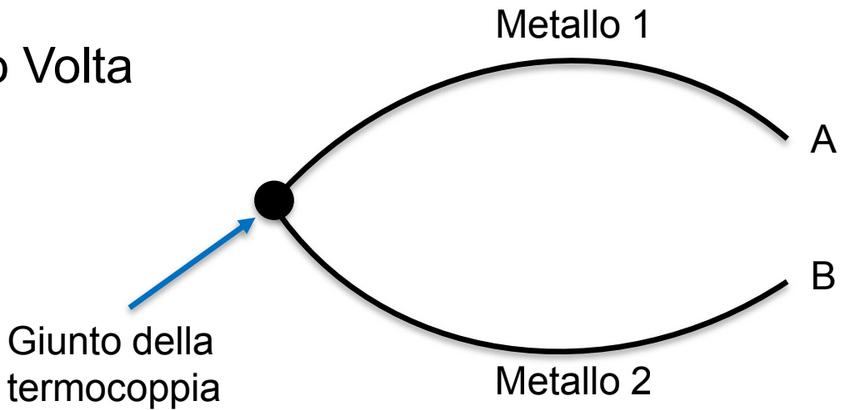
\includegraphics[width=5cm]{eff-volta}
			\caption{schema di riferimento per l'effetto Volta.}
		\end{SCfigure}
		
		\item l'\textbf{effetto Seebeck} invece considera il flusso di elettroni in catena chiusa; in particolare considerando due fili metallici collegati in due giunzioni poste a temperature $T_1,T_2$; nel caso in cui le due temperature fossero diverse ($T_1\neq T_2$) si osserverebbe che all'interno della catena chiusa gli elettroni inizierebbero a circolare, determinando di fatto una corrente elettrica;
	
		\begin{SCfigure}[1][bht]
			\centering
			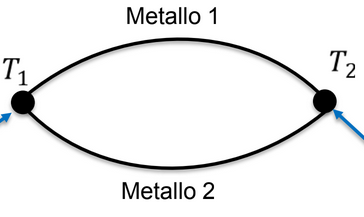
\includegraphics[width=5cm]{eff-seebeck}
			\caption{schema di riferimento per l'effetto Seebeck.}
		\end{SCfigure}
	\end{itemize}

	L'idea alla base dell'utilizzo delle termocoppie è proprio quella di rilevare la differenza di tensione generata tra i due giunti, osservando che tale valore dipenderà sicuramente dalla temperatura differenziale.

	\begin{SCfigure}[0.7][bht]
		\centering
		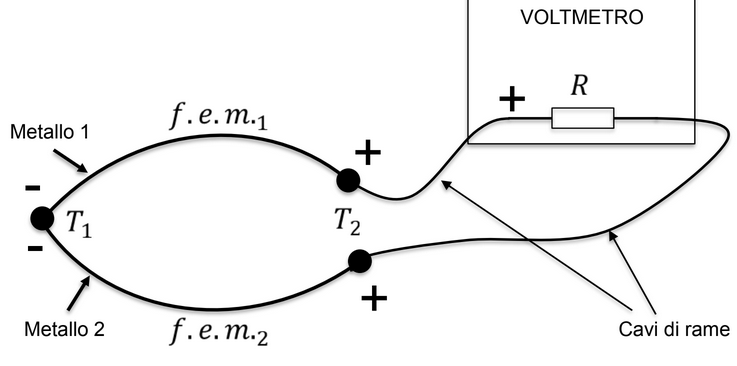
\includegraphics[width=8cm]{termocoppia-1}
		\caption{implementazione di una termocoppia.}
		\label{fig:termocoppia:schema}
	\end{SCfigure}
	
	Facendo riferimento alla realizzazione di una termocoppia mostrata in figura \ref{fig:termocoppia:schema}, è possibile osservare come la tensione rilevata dal voltmetro, rappresentata dalla forza elettromotrice generata dalla termocoppia $fem_{t.c.}$, dipende necessariamente dalle forze elettromotrici generate dai due cavi secondo la relazione
	\begin{equation} \label{eq:termocoppia:base}
		fem_{t.c.} = fem_1 - fem_2
	\end{equation}

	A questo punto si osserva che se i giunti si trovano a temperature uguali ($T_1 = T_2$) allora le forze elettromotrici generate dai due metalli sono uguali, pertanto 
	\[ T_1 = T_2 \qquad \Rightarrow \quad fem_1 = fem_2 \qquad \Rightarrow \quad fem_{t.c.} = 0  \]
	
	Al contrario se le temperatura dei giunti sono diverse ($T_1\neq T_2$) allora le forze elettromotrici sui due cavi sono diverse, e questo comporta una tensione differenziale in uscita dalla termocoppia che può essere valutata dal voltmetro:
	\[ T_1 \gtrless T_2  \qquad \Rightarrow \quad fem_1 \gtrless fem_2 \qquad \Rightarrow \quad fem_{t.c.} \gtrless 0 \]
	
	\subsection{Altri effetti termoelettrici}
		Parlando di termocoppie è necessario anche considerare anche altri effetti termoelettrici che si instaurano nel sistema in esame. In particolare l'\textbf{effetto Peltier}, duale all'effetto Seebeck, afferma che se una termocoppia è soggetta ad un passaggio di corrente, allora sul giunto della stessa si avrà un processo di emissione/assorbimento di calore. Nella pratica questo tipo di effetto può essere trascurato nella misurazione in quanto non rilevante.
		
		Più rilevante può essere invece l'\textbf{effetto Thompson} che considera un'eventuale emissione/assorbimento di calore ed è dovuto alla possibile variazione del coefficiente Seebeck in funzione della temperatura lungo un filo. Tale tipo di effetto si può considerare come un effetto Peltier distribuito lungo tutta la lunghezza dei cavi che porta a riscrivere l'equazione \ref{eq:termocoppia:base} tramite la formulazione
		\begin{equation}
			fem_{t.c.} = \underbrace{c_1 \big(T_1-T_2\big)}_\textrm{Seebeck} +\underbrace{ c_2\big(T_1^2-T_2^2\big)}_\textrm{Thomson}
		\end{equation}
		dove $c_1$ è il coefficiente legato all'effetto Seebeck e $c_2$ quello legato all'effetto Thompson e in generale tali valori sono forniti dal produttore sulla base di analisi sperimentali.

	\subsection{Proprietà delle termocoppie}
	
		Una prima proprietà fondamentale delle termocoppie è basata sul fatto che la differenza di tensione $e_u$ rilevata ai giunti della termocoppia dipende solamente dalla differenza di temperatura dei giunti stessi, ed è indipendente in ogni modo indipendente dalla temperatura sui fili (nei quali in generale essa può cambiare).
	
		\begin{SCfigure}[2][bht]
			\centering
			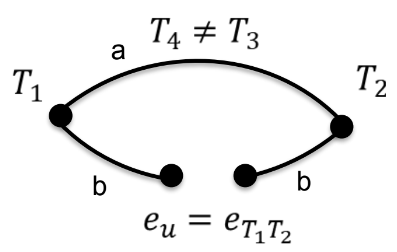
\includegraphics[width=4cm]{tc-prop-1}
			\caption{in una termocoppia la differenza di potenziale $e_u$ rilavata dipende solamente dalla differenza di temperatura dei due giunti.}
		\end{SCfigure}
		
		Un'altra proprietà di rilevante interesse pratico è quella che ci permette di affermare che interponendo nella termocoppia un terzo cavo metallico (come in figura \ref{fig:termocoppia:prop2}) i cui giunti con i metalli originari sono posti ad una temperatura uguale, allora la tensione differenziale rilevata dalla termocoppia rimane invariata. Questo è particolarmente utile dal punto di vista applicativo in quanto permette di effettuare la trasmissione dei segnali mediante cavi meno costosi rispetto a quelli utilizzati per la termocoppia vera e propria (che di norma sono costosi in quanto leghe molto difficili da ricavare).
		
		\begin{SCfigure}[2][bht]
			\centering
			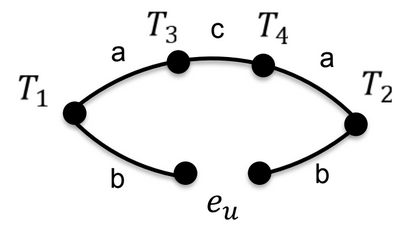
\includegraphics[width=4cm]{tc-prop-2}
			\caption{interponendo un terzo cavo metallico $c$ all'interno della termocoppia, se le temperature dei due nuovi giunti è uguale allora la differenza di tensione rilevata dalla termocoppia è invariante.}
			\label{fig:termocoppia:prop2}
		\end{SCfigure}
		
		Un'altra importante proprietà è quella che ci permette di tarare la termocoppia: si osserva infatti che noto il potenziale $e_c$ generato da un metallo di una termocoppia, è possibile tarare gli altri metalli combinando i vari risultati sperimentali, ossia in generale non è necessario tarare singolarmente ogni coppia di conduttori ma è sufficiente considerare le tensioni differenziali generate (come in figura \ref{fig:termocoppia:prop3}).
		
		\begin{figure}[bht]
			\centering
			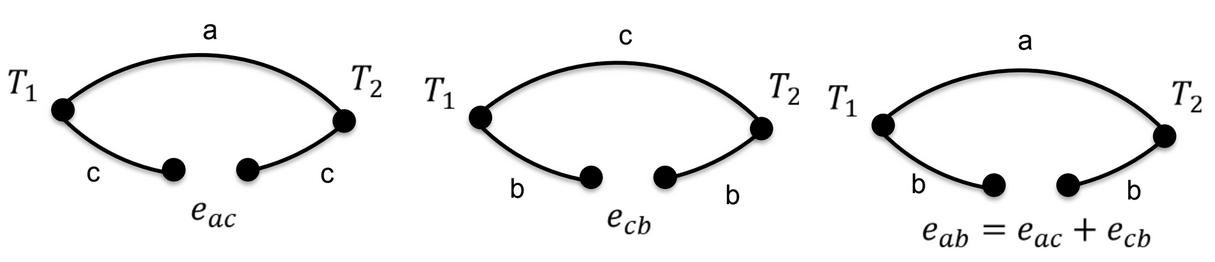
\includegraphics[width=10cm]{tc-prop-4}
			\caption{ogni termocoppia può essere tarata a partire da un metallo di riferimento.}
			\label{fig:termocoppia:prop3}
		\end{figure}
		
	\subsection{Utilizzo delle termocoppie}
		A questo punto avendo visto che l'intromissione di cavi per il trasporto del segnale non influiscono sul segnale letto dal microvoltmetro (se la temperatura dei giunti due nuovi giunti è uguale), allora è possibile pensare di realizzare una vera e propria termocoppia di utilità pratica.
		
		\begin{figure}[bht]
			\centering
			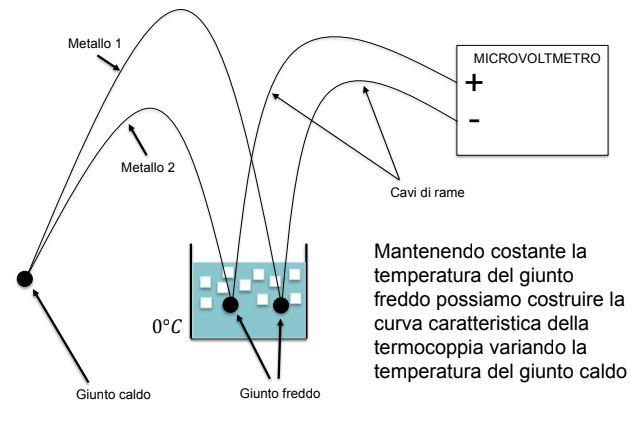
\includegraphics[width=9cm]{termocoppia-schema}
			\caption{implementazione di una coppia termoelettrica nella pratica.}
			\label{fig:termocoppia}
		\end{figure}
	
		Uno strumento di misura basato sulla termocoppia è esemplificato in figura \ref{fig:termocoppia} dove è possibile osservare come uno dei due giunti è posto ad una sorgente calda da valutare, mentre il secondo giunto è posto in un ambiente freddo a temperatura nota (e rispetto a tale punto parte anche il cavo di trasmissione delle informazioni). In questo modo, nota la temperatura del giunto freddo e potendo stabilire la temperatura differenziale tra i giunti mediante la caratteristica statica letta dal microvoltmetro, allora è possibile stabilire la temperatura del giunto caldo oggetto di studio.
		
		\paragraph{Materiali} In generale le termocoppie sono realizzate in materiali molto costosi per via delle loro proprietà; in particolare tali materiali sono classificati in vari tipi (le cui proprietà sono mostrate in figura \ref{fig:termocoppia:caratteristica}) in funzione della sensibilità della coppia metallica e del range di temperatura in cui può essere utilizzato. 	
		
		\begin{figure}[bht]
			\centering
			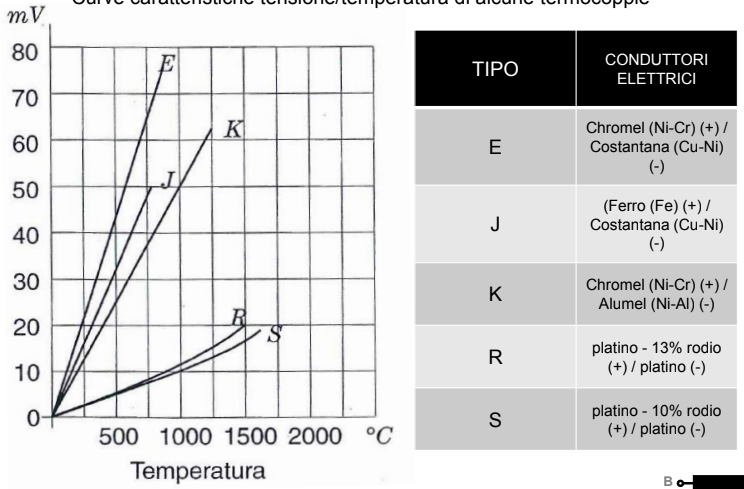
\includegraphics[width=9cm]{termocoppia-caratteristica}
			\caption{caratteristica statica di varie categorie di termocoppie.}
			\label{fig:termocoppia:caratteristica}
		\end{figure}
			
		Per via del compromesso tra range di temperatura e sensibilità (ma soprattutto della linearità della caratteristica statica) dello strumento di misura, il tipo di termocoppia più utilizzato è quello di tipo $K$.
		
		\vspace{3mm}
		
		Essendo in generale i metalli costosi, nella pratica si utilizzando i metalli sopra citati solamente nei punti esposti alle alte temperature che si vogliono misurare, mentre al di fuori di tale zona critica si utilizzando dei cosiddetti \textbf{cavi compensati}, ossia cavi metallici caratterizzati da avere potenziale di estrazione pari al metallo utilizzato nella termocoppia, ma realizzati con materiali meno costosi, diminuendo il costo complessivo dello strumento di misura.
		
	
\section{Termoresistenze}
	Le termoresistenze si basano sul fatto che la resistenza $R$ di un metallo è funzione delle temperatura $T$ cui esso è sottoposto; per esempio è possibile calcolare la resistenza in funzione dell'intervallo di temperatura secondo le leggi
	\[ R(T_{^\circ C}) = \begin{cases}
		R_0\big(1 + aT + bT^2 + c(T-100)^3\big) \qquad & T\in [-200^\circ C, 0^\circ C] \\
		R_0\big(1 + aT + bT^2\big) \qquad &T\in [0^\circ C,850^\circ C] 
	\end{cases}\]
	dove la temperatura $T$ è espressa in gradi Celsius, $R_0$ è la resistenza del conduttore alla temperatura $0^\circ C$ e $a,b,c$ sono dei coefficienti del metallo.
	
	Per la realizzazione di termoresistenze in generale si utilizzano nickel, rame e platico; in particolare noi facciamo riferimento alla sonda \texttt{PT100} realizzata in platino con resistenza $R_0 = 100 \Omega$ con classe di accuratezza $A$ (più accurata) e $B$ (meno accurata).
	
	Per disaccoppiare dall'effetto di temperatura quello di deformazione si avvolge il filo a spirale e si immerge il metallo in una polvere di allumina che isola dalle vibrazioni pur conducendo calore (in questo modo si elimina l'effetto \textit{estensimetro}).
	
	Trascurando la resistenza dei fili di collegamento tra termoresistenza e apparato di misurazione, la temperatura viene misurata tramite un ponte di Wheatstone semplice. Il trascurare i cavi può portare a grossi errori in quanto aumentano la resistenza equivalente del circuito e la temperatura dei fili può modificare la temperatura che si vuole misurare. Per ovviare a questo problema, come per gli estensimetri, si effettua un collegamento a tre fili con il ponte di Wheatstone
	
	\textbf{AGGIUNGERE LE FIGURE} 
	
	Un altro problema del circuito è dovuto alla bassa resistenza della sonda; in generale dovendo essere pari a $20mA$ la corrente massima che può scorrere sull circuito, considerando le due resistenze $R_1,R_2= 100\Omega$ la tensione di alimentazione è limitata al valore
	\[ V= I_{max} R_{eq} = 4V \]
	
	Un modo per ovviare a questo problema è di porre a $25V$ la tensione di alimentazione da modulare con un duty cycle in modo che la tensione media nel tempo è di $4V$.
	
	Un altro metodo di misurazione è quello \textbf{volt-amperometrico} con collegamento a due fili; in questo caso il circuito è alimentato da un generatore di corrente e, tramite un multimetro, si misura la differenza di tensione ai capi dei due fili. In questo caso l'uscita non è proporzionale solamente alla resistenza della sonda, ma anche a quella dei fili. \\
	Per ridurre questo problema si utilizza lo stesso metodo ma a 4 fili
	
	
	
\section{Noise thermometers}
	I \de{noise termometers} fa parte dei metodi alternativi di misurazione della temperatura.  Questi strumenti si basano sulla stima del rumore (dovuto alla temperatura) correlato alla temperatura del misurando tramite stima della deviazione standard. Questo strumento si basa sul fatto che il \textit{rumore} è detto \textit{bianco} in quanto ogni componente in frequenza è presente con un modulo pressoché equivalente.
	
	
	Misurando la tensione media dovuto a questo rumore si evince che essa è nulla in quanto $V_m = \frac 1 t \int_0 ^t V(\xi)\, d\xi =0$, mentre lo scarto quadratico medio si può osservare non essere nullo $\sigma^2 = \frac 1 t \int_0 ^t V^2 (\xi)\, d\xi \neq 0$.
	
	
\section{Pirometri ad infrarosso}
	I \de{pirometri ad infrarosso} si basano sulla misura pirometrica, ossia sul rilevare la radiazione elettromagnetica propria emessa dal corpo misurando; questo è dunque un sistema di misura senza contatto tra misurando e sistema di misura. 
	
	In particolare tramite la legge di Plank è possibile misurare la potenza $W$ trasmessa da un corpo nero in funzione della lunghezza d'onda $\lambda$ (in $\mu m$) e della temperatura $T$ (in gradi Kelvin) secondo l'equazione
	\[ W(\lambda, T) =  \frac{ c_1  }{\lambda^5\left(e^{c_2/\lambda T} - 1\right)}\]
	Per integrazione della potenza per unità di lunghezza rispetto allo spettro di frequenza è possibile calcolare la potenza totale irradiata dal corpo: $P = \int_\lambda W(\lambda, T)\, d\lambda$. Osservando che la lunghezza d'onda di picco segue un'equazione del tipo $\lambda_\textrm{picco} = 2891/T$, per integrazione si ricava che pa potenza è una potenza quarta della temperatura:
	\[ P =\int_\lambda W(\lambda, T)\, d\lambda = 5.67  \cdot 10^{-12} T^4 \]
	
	Per i \textbf{corpi reali} il comportamento risulta essere leggermente diverso rispetto a quello ideale del corpo nero: si parla di \textit{corpo grigio} se lo spettro è attenuato di un valore costante (inferiore al valore unitario), mentre un \textit{corpo} è detto \textit{colorato} se l'attenuazione dipende dalla lunghezza d'onda che si vuole rilevare. In generale la relazione è espressa dalla funzione
	\[ W_a(\lambda, T) =\frac{\varepsilon(\lambda,T) c_1}{\lambda^5\left(e^{c_2/\lambda T} - 1\right)} \]
	dove $\varepsilon(\lambda, T) \in [0,1]$ è l'\textbf{emissività} del corpo. Tale fattore dipende, oltre che da $\lambda$ e $T$, anche dalla rugosità della superficie, dall'angolo rispetto al quale si effettua la rilevazione... 
	
	Un problema legato a questo tipo di misuratore è che lo stesso rileva anche le radiazioni riflette da altri corpi sul corpo oggetto di misura.
	
	